\section{Równania różniczkowe cząstkowe I i II rzędu}
\subsection{Równania różniczkowe liniowe rzędu II}
Równanie różniczkowe postaci:
$$ a(x,y) \dfrac{\partial^2u}{\partial x^2} + 2b \dfrac{\partial ^2u}{\partial x \partial u} + c(x,y)\dfrac{\partial^2u}{\partial y^2} + d(x,y) \dfrac{\partial u}{\partial x} + e(x,y) \dfrac{\partial u}{\partial y} + f(x,y) u + g(x,y) = 0$$

nazywamy równaniem różniczkowym cząstkowym liniowym rzędu II, gdzie $a^2 + b^2 + c^2>0$ na $\Omega$,\\ a, b, c, d, e, f, g $\in$ C($\Omega$)
\\
\\
Wyróżnik równania cząstkowego rzędu II:
$$\Delta = b^2 = ac$$\\
Równanie różniczkowe cząstkowe liniowe rzędu II jest typu eliptycznego, gdy $\Delta < 0$

\subsection{Cel ćwiczenia}
Naszym zadaniem było rozwiązanie równań Laplace'a i Poissona z dwuwymiarowymi zagadnieniami Dirichletta za pomocą stworzonego przez nas programu.
\\
\\
Równanie Poissona z dwuwymiarowymi zagadnieniami Dirichletta jest równaniem eliptycznym postaci:
\[
\begin{cases}
\vspace{0.1cm} 
\hspace{0,1cm}\dfrac{\partial^2 u}{\partial x^2} + \dfrac{\partial^2 u}{\partial y^2} = f\\
\vspace{0.1cm}
\hspace{0,1cm}u_{|\partial \Omega} = \widetilde{u} \\
\end{cases}
\]

, gdzie:

$(x,y) \in \Omega$

$\Omega = [a,b] \times [c,d]$

$\Omega \subset \Re^2$

Postać równania Laplace'a otrzymujemy przez podstawienie do równania Poissona $f \equiv 0$. \\

Wykorzystując schemat 5-pkt. dla operatora Laplace'a otrzymujemy odpowiednie równania:\\

\begin{enumerate}
	\item Dla siatki równomiernej (h=k)
	\begin{equation}
-4u_{i,j} + u_{i+1,j} + u_{i-1,j} + u_{i,j+1} + u_{i,j-1} = h^2 f_{i,j} \tag{*}
	\end{equation}
	
	\item Dla siatki nierównomiernej (h $\neq$ k)
	\begin{equation}
		\dfrac{1}{h^2}\left(u_{i+1,j} + u_{i-1,j} \right) + \dfrac{1}{k^2} \left(u_{i,j+1} + u_{i,j-1} \right) -2\left(\dfrac{1}{h^2} + \dfrac{1}{k^2} \right)u_{i,j} = f_{i,j} \tag{**}
	\end{equation}	
\end{enumerate}
Stosując równanie (**) otrzymujemy ogólniejsze rozwiązanie, ponieważ równienie (*) otrzymujemy przez podstawnie $k=h$ oraz odpowiednie przekształcenia.
\\	

Rozwiązaliśmy następujące równania:
\begin{multicols}{3}
	a)\\\\$\dfrac{\partial^2 u}{\partial x^2} + \dfrac{\partial^2 u}{\partial y^2} = 0$\vspace{0.2cm}\\\\, gdzie:\\
	$\Omega = [0,1]\times[0,1]$\\
	warunki brzegowe:\\
	$u(x,0) = 0$\\
	$u(1,y) = y$\\
	$u(x,1) = x$\\
	$u(0,y) = 0$
	\vspace{0.1cm}\\
	Rozwiązanie analityczne:\\
	\columnbreak
	$\widetilde{u}(x,y) = xy$\\
	b)\\\\$\dfrac{\partial^2 u}{\partial x^2} + \dfrac{\partial^2 u}{\partial y^2} = (x^2+y^2)e^{xy}$\vspace{0.2cm}\\\\, gdzie:\\
	$\Omega = [0,2]\times[0,1]$\\
	warunki brzegowe:\\
	$u(x,0) = 1$\\
	$u(2,y) = e^{2y}$\\
	$u(x,1) = e^x$\\	
	$u(0,y) = 1$
	\vspace{0.1cm}\\
	Rozwiązanie analityczne:\\
	\columnbreak
	$\widetilde{u}(x,y) = e^{xy}$\\
	c)\\\\$\dfrac{\partial^2 u}{\partial x^2} + \dfrac{\partial^2 u}{\partial y^2} = \dfrac{x}{y} + \dfrac{y}{x}$\vspace{0cm}\\\\, gdzie:\\
	$\Omega = [1,2]\times[1,2]$\\
	warunki brzegowe:\\
	$u(x,1) = x\cdot lnx$\\
	$u(2,y) = 2y\cdot ln(2y)$\\
	$u(x,2) = x\cdot ln(4x^2)$\\
	$u(1,y) = y\cdot lny$
	\vspace{0.1cm}\\
	Rozwiązanie analityczne:\\
	$\widetilde{u}(x,y) = xy\cdot ln(xy)$
	
	
\end{multicols}

\subsection{Algorytm}

\begin{samepage}
%\begin{Shaded}
\begin{Highlighting}[]
\FunctionTok{clear}\NormalTok{, }\FunctionTok{clc}\NormalTok{;}
\CommentTok{% zad 3}
\CommentTok{% Przykładowe dane}
\NormalTok{nx = }\FloatTok{10}\NormalTok{; ny = }\FloatTok{10}\NormalTok{; xa = }\FloatTok{0}\NormalTok{; xb = }\FloatTok{2}\NormalTok{; ya = }\FloatTok{0}\NormalTok{; yb = }\FloatTok{1}\NormalTok{;}
\NormalTok{f = @(x, y) (x.^}\FloatTok{2} \NormalTok{+ y.^}\FloatTok{2}\NormalTok{) .* }\FunctionTok{exp}\NormalTok{(x.*y);}
\NormalTok{g = @(x, y) }\FunctionTok{exp}\NormalTok{(x.*y);}
\NormalTok{uxa = @(x) }\FloatTok{1}\NormalTok{;         }\CommentTok{%u1}
\NormalTok{uxb = @(x) }\FunctionTok{exp}\NormalTok{(x);    }\CommentTok{%u3}
\NormalTok{uya = @(y) }\FloatTok{1}\NormalTok{;         }\CommentTok{%u4}
\NormalTok{uyb = @(y) }\FunctionTok{exp}\NormalTok{(}\FloatTok{2}\NormalTok{.*y); }\CommentTok{%u2}

\CommentTok{% Obliczenia}
\NormalTok{h = (xb-xa)/(nx+}\FloatTok{1}\NormalTok{);}
\NormalTok{k = (yb-ya)/(ny+}\FloatTok{1}\NormalTok{);}
\NormalTok{xM = }\FunctionTok{linspace}\NormalTok{(xa + h, xb - h, nx);}
\NormalTok{yM  = }\FunctionTok{linspace}\NormalTok{(ya+k, yb-k, ny);}
\NormalTok{T = -}\FloatTok{4}\NormalTok{* }\FunctionTok{eye}\NormalTok{(nx) + }\FunctionTok{diag}\NormalTok{(}\FunctionTok{diag}\NormalTok{(}\FunctionTok{eye}\NormalTok{(nx-}\FloatTok{1}\NormalTok{)),-}\FloatTok{1}\NormalTok{) + }\FunctionTok{diag}\NormalTok{(}\FunctionTok{diag}\NormalTok{(}\FunctionTok{eye}\NormalTok{(nx-}\FloatTok{1}\NormalTok{)),}\FloatTok{1}\NormalTok{);}
\BaseNTok{I} \NormalTok{= }\FunctionTok{eye}\NormalTok{(nx);}
\NormalTok{B = }\FunctionTok{kron}\NormalTok{(}\FunctionTok{eye}\NormalTok{(ny), T);}
\NormalTok{C = }\FunctionTok{kron}\NormalTok{(}\FunctionTok{diag}\NormalTok{(}\FunctionTok{diag}\NormalTok{(}\FunctionTok{eye}\NormalTok{(ny-}\FloatTok{1}\NormalTok{)),-}\FloatTok{1}\NormalTok{), }\BaseNTok{I}\NormalTok{);}
\NormalTok{D = }\FunctionTok{kron}\NormalTok{(}\FunctionTok{diag}\NormalTok{(}\FunctionTok{diag}\NormalTok{(}\FunctionTok{eye}\NormalTok{(ny-}\FloatTok{1}\NormalTok{)),}\FloatTok{1}\NormalTok{), }\BaseNTok{I}\NormalTok{);}
\NormalTok{A = B + C + D;}

\NormalTok{[X1 Y1] = }\FunctionTok{meshgrid}\NormalTok{(xM,yM);}
\NormalTok{F = f(X1, Y1)' .* }\FunctionTok{ones}\NormalTok{(nx, ny);}
\NormalTok{F = h^}\FloatTok{2} \NormalTok{.* F;}
\NormalTok{F(:, }\FloatTok{1}\NormalTok{) = F(:, }\FloatTok{1}\NormalTok{) - uxa(xM)';}
\NormalTok{F(:, ny) = F(:, ny) - uxb(xM)';}
\NormalTok{F(}\FloatTok{1}\NormalTok{, :) = F(}\FloatTok{1}\NormalTok{, :) - uya(yM);}
\NormalTok{F(nx, :) = F(nx, :) - uyb(yM);}
\NormalTok{F = }\FunctionTok{reshape}\NormalTok{(F,  nx*ny, }\FloatTok{1}\NormalTok{);}
\CommentTok{% Rozwiązanie}
\NormalTok{U = linsolve(A,F);}
\NormalTok{U = }\FunctionTok{reshape}\NormalTok{(U,  nx, ny)';}
\NormalTok{[X,Y] = }\FunctionTok{meshgrid}\NormalTok{(xa:h:xb, ya:k:yb);}
\NormalTok{U = [uya(yM)' .* }\FunctionTok{diag}\NormalTok{(}\FunctionTok{eye}\NormalTok{(ny)), U, uyb(yM)' .* }\FunctionTok{diag}\NormalTok{(}\FunctionTok{eye}\NormalTok{(ny))];}
\NormalTok{XM = [xa xM xb];}
\NormalTok{G = g(X,Y);}
\NormalTok{U = [uxa(XM)' .* }\FunctionTok{diag}\NormalTok{(}\FunctionTok{eye}\NormalTok{(nx+}\FloatTok{2}\NormalTok{)), U', uxb(XM)' .* }\FunctionTok{diag}\NormalTok{(}\FunctionTok{eye}\NormalTok{(nx+}\FloatTok{2}\NormalTok{))]';}
\CommentTok{% Błąd}
\NormalTok{Error = }\FunctionTok{max}\NormalTok{(}\FunctionTok{max}\NormalTok{(}\FunctionTok{abs}\NormalTok{(G-U)));}
\CommentTok{% Wykres}
\FunctionTok{subplot}\NormalTok{(}\FloatTok{1}\NormalTok{,}\FloatTok{2}\NormalTok{,}\FloatTok{1}\NormalTok{)}
\FunctionTok{surf}\NormalTok{(X,Y,U)}
\FunctionTok{subplot}\NormalTok{(}\FloatTok{1}\NormalTok{,}\FloatTok{2}\NormalTok{,}\FloatTok{2}\NormalTok{)}
\FunctionTok{surf}\NormalTok{(X,Y,G)}
\end{Highlighting}
\end{Shaded}
 złe zmienić na nowe!
\begin{Shaded}
\begin{Highlighting}[]
\FunctionTok{clear}\NormalTok{, }\FunctionTok{clc}\NormalTok{;}
\CommentTok{% zad 2}
\CommentTok{% Przykładowe dane}
\NormalTok{nx = }\FloatTok{10}\NormalTok{; ny = }\FloatTok{50}\NormalTok{; xa = }\FloatTok{0}\NormalTok{; xb = }\FloatTok{2}\NormalTok{; ya = }\FloatTok{0}\NormalTok{; yb = }\FloatTok{1}\NormalTok{;}
\NormalTok{f = @(x, y) (x.^}\FloatTok{2}\NormalTok{ + y.^}\FloatTok{2}\NormalTok{) .* }\FunctionTok{exp}\NormalTok{(x.*y);}
\NormalTok{g = @(x, y) }\FunctionTok{exp}\NormalTok{(x.*y);}
\NormalTok{uxa = @(x) }\FloatTok{1}\NormalTok{;         }\CommentTok{%u1}
\NormalTok{uxb = @(x) }\FunctionTok{exp}\NormalTok{(x);    }\CommentTok{%u3}
\NormalTok{uya = @(y) }\FloatTok{1}\NormalTok{;         }\CommentTok{%u4}
\NormalTok{uyb = @(y) }\FunctionTok{exp}\NormalTok{(}\FloatTok{2}\NormalTok{.*y); }\CommentTok{%u2}

\CommentTok{% Obliczenia}
\NormalTok{h = (xb-xa)/(nx+}\FloatTok{1}\NormalTok{);}
\NormalTok{k = (yb-ya)/(ny+}\FloatTok{1}\NormalTok{);}
\NormalTok{xM = }\FunctionTok{linspace}\NormalTok{(xa + h, xb - h, nx);}
\NormalTok{yM  = }\FunctionTok{linspace}\NormalTok{(ya+k, yb-k, ny);}
\NormalTok{T = -}\FloatTok{2}\NormalTok{*(h^}\FloatTok{2}\NormalTok{ + k^}\FloatTok{2}\NormalTok{) * }\FunctionTok{eye}\NormalTok{(nx) + k^}\FloatTok{2}\NormalTok{ * }\FunctionTok{diag}\NormalTok{(}\FunctionTok{diag}\NormalTok{(}\FunctionTok{eye}\NormalTok{(nx-}\FloatTok{1}\NormalTok{)),-}\FloatTok{1}\NormalTok{) \textbackslash{}}
\NormalTok{+ k^}\FloatTok{2}\NormalTok{ * }\FunctionTok{diag}\NormalTok{(}\FunctionTok{diag}\NormalTok{(}\FunctionTok{eye}\NormalTok{(nx-}\FloatTok{1}\NormalTok{)),}\FloatTok{1}\NormalTok{);}
\BaseNTok{I}\NormalTok{ = }\FunctionTok{eye}\NormalTok{(nx);}
\NormalTok{B = }\FunctionTok{kron}\NormalTok{(}\FunctionTok{eye}\NormalTok{(ny), T);}
\NormalTok{C = }\FunctionTok{kron}\NormalTok{(}\FunctionTok{diag}\NormalTok{(}\FunctionTok{diag}\NormalTok{(}\FunctionTok{eye}\NormalTok{(ny-}\FloatTok{1}\NormalTok{)),-}\FloatTok{1}\NormalTok{), h^}\FloatTok{2}\NormalTok{ * }\BaseNTok{I}\NormalTok{);}
\NormalTok{D = }\FunctionTok{kron}\NormalTok{(}\FunctionTok{diag}\NormalTok{(}\FunctionTok{diag}\NormalTok{(}\FunctionTok{eye}\NormalTok{(ny-}\FloatTok{1}\NormalTok{)),}\FloatTok{1}\NormalTok{), h^}\FloatTok{2}\NormalTok{ * }\BaseNTok{I}\NormalTok{);}
\NormalTok{A = B + C + D;}

\NormalTok{[X1 Y1] = }\FunctionTok{meshgrid}\NormalTok{(xM,yM);}
\NormalTok{F = f(X1, Y1)' .* }\FunctionTok{ones}\NormalTok{(nx, ny);}
\NormalTok{F = h^}\FloatTok{2}\NormalTok{ * k^}\FloatTok{2}\NormalTok{ .* F;}
\NormalTok{F(:, }\FloatTok{1}\NormalTok{) = F(:, }\FloatTok{1}\NormalTok{) - h^}\FloatTok{2}\NormalTok{ * uxa(xM)';}
\NormalTok{F(:, ny) = F(:, ny) - h^}\FloatTok{2}\NormalTok{ * uxb(xM)';}
\NormalTok{F(}\FloatTok{1}\NormalTok{, :) = F(}\FloatTok{1}\NormalTok{, :) - k^}\FloatTok{2}\NormalTok{ * uya(yM);}
\NormalTok{F(nx, :) = F(nx, :) - k^}\FloatTok{2}\NormalTok{ * uyb(yM);}
\NormalTok{F = }\FunctionTok{reshape}\NormalTok{(F,  nx*ny, }\FloatTok{1}\NormalTok{);}
\CommentTok{% Rozwiązanie}
\NormalTok{U = linsolve(A,F);}
\NormalTok{U = }\FunctionTok{reshape}\NormalTok{(U,  nx, ny)';}
\NormalTok{[X,Y] = }\FunctionTok{meshgrid}\NormalTok{(xa:h:xb, ya:k:yb);}
\NormalTok{U = [uya(yM)' .* }\FunctionTok{diag}\NormalTok{(}\FunctionTok{eye}\NormalTok{(ny)), U, uyb(yM)' .* }\FunctionTok{diag}\NormalTok{(}\FunctionTok{eye}\NormalTok{(ny))];}
\NormalTok{XM = [xa xM xb];}
\NormalTok{G = g(X,Y);}
\NormalTok{U = [uxa(XM)' .* }\FunctionTok{diag}\NormalTok{(}\FunctionTok{eye}\NormalTok{(nx+}\FloatTok{2}\NormalTok{)), U', uxb(XM)' .* }\FunctionTok{diag}\NormalTok{(}\FunctionTok{eye}\NormalTok{(nx+}\FloatTok{2}\NormalTok{))]';}
\CommentTok{% Błąd}
\NormalTok{Error = }\FunctionTok{max}\NormalTok{(}\FunctionTok{max}\NormalTok{(}\FunctionTok{abs}\NormalTok{(G-U)));}
\CommentTok{% Wykres}
\FunctionTok{subplot}\NormalTok{(}\FloatTok{1}\NormalTok{,}\FloatTok{2}\NormalTok{,}\FloatTok{1}\NormalTok{)}
\FunctionTok{surf}\NormalTok{(X,Y,U)}
\FunctionTok{subplot}\NormalTok{(}\FloatTok{1}\NormalTok{,}\FloatTok{2}\NormalTok{,}\FloatTok{2}\NormalTok{)}
\FunctionTok{surf}\NormalTok{(X,Y,G)}
\end{Highlighting}
\end{Shaded}
\end{samepage}

\newpage

\subsection{Wykresy}

a)

Dla nx = ny = 5:

\begin{figure}[!ht]
	\begin{center}
		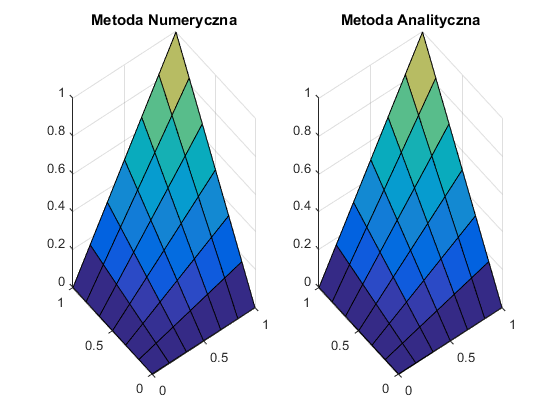
\includegraphics[width=0.78\textwidth]{Lab5/charts/zad1/5x5.png}
	\end{center}
\end{figure}

Czas wykonywania algorytmu $ = 0.0136 s$

Dla nx = ny = 15:

\begin{figure}[!ht]
	\begin{center}
		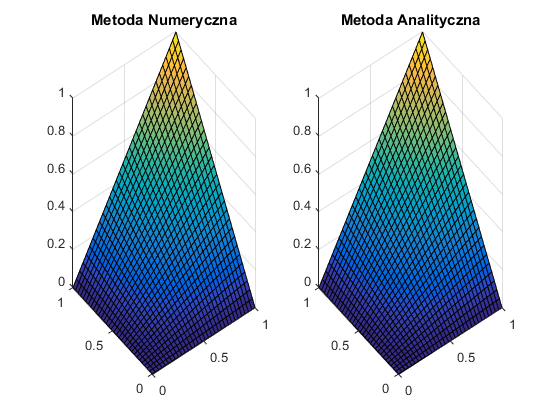
\includegraphics[width=0.78\textwidth]{Lab5/charts/zad1/15x15.png}
	\end{center}
\end{figure}

Czas wykonywania algorytmu $ = 0.0155 s$

\newpage
Dla nx = ny = 30:

\begin{figure}[!ht]
	\begin{center}
		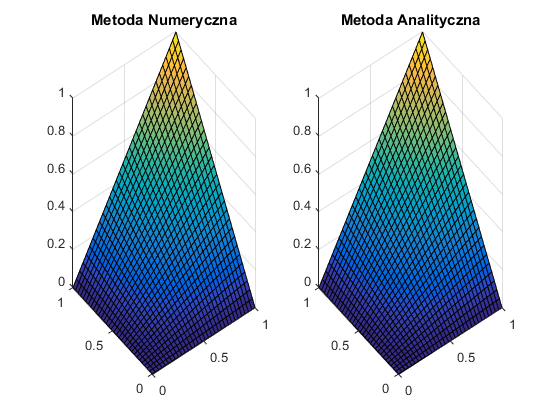
\includegraphics[width=0.8\textwidth]{Lab5/charts/zad1/30x30.png}
	\end{center}
\end{figure}

Czas wykonywania algorytmu $ = 0.0329 s$

Dla nx = ny = 100:

\begin{figure}[!ht]
	\begin{center}
		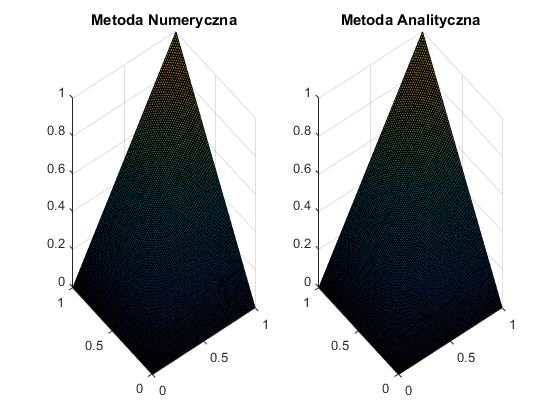
\includegraphics[width=0.8\textwidth]{Lab5/charts/zad1/100x100.png}
	\end{center}
\end{figure}

Czas wykonywania algorytmu $ = 6,370 s$

\newpage

Błąd metody w zależności od liczby węzłów:

\begin{figure}[!ht]
	\begin{center}
		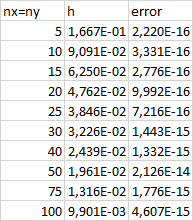
\includegraphics[width=0.8\textwidth]{Lab5/charts/zad1/error_dane.png}
	\end{center}
\end{figure}

\begin{figure}[!ht]
	\begin{center}
		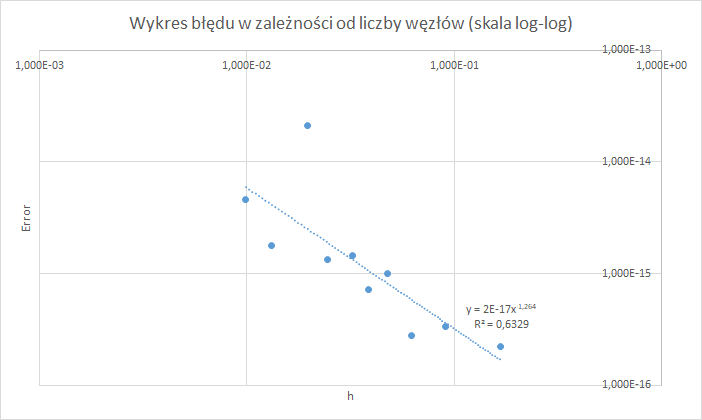
\includegraphics[width=0.8\textwidth]{Lab5/charts/zad1/error.png}
	\end{center}
\end{figure}

\newpage

b)

Dla nx = ny = 5:

\begin{figure}[!ht]
	\begin{center}
		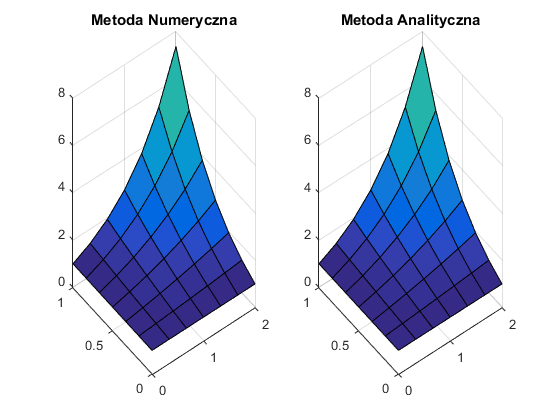
\includegraphics[width=0.78\textwidth]{Lab5/charts/zad2/5x5.png}
	\end{center}
\end{figure}

Czas wykonywania algorytmu $ = 0.0140 s$

Dla nx = ny = 15:

\begin{figure}[!ht]
	\begin{center}
		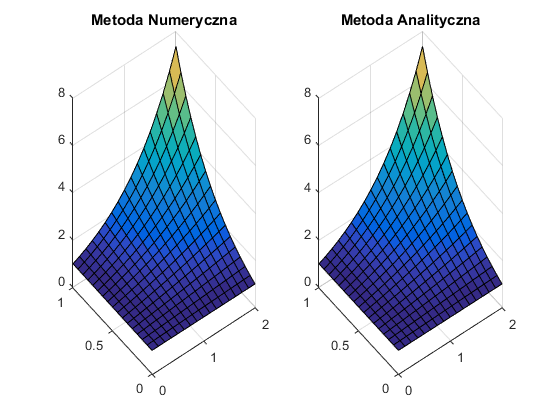
\includegraphics[width=0.78\textwidth]{Lab5/charts/zad2/15x15.png}
	\end{center}
\end{figure}

Czas wykonywania algorytmu $ = 0.0157 s$

\newpage
Dla nx = ny = 30:

\begin{figure}[!ht]
	\begin{center}
		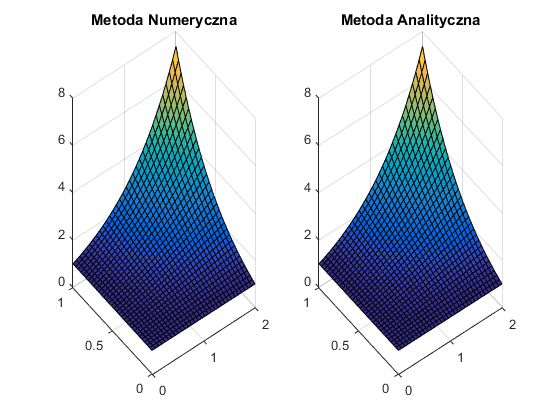
\includegraphics[width=0.8\textwidth]{Lab5/charts/zad2/30x30.png}
	\end{center}
\end{figure}

Czas wykonywania algorytmu $ = 0.0320 s$

Dla nx = ny = 100:

\begin{figure}[!ht]
	\begin{center}
		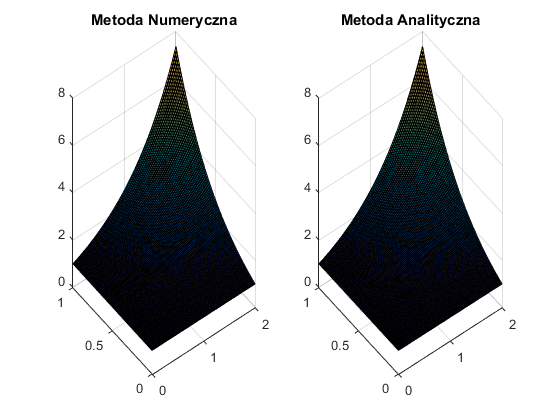
\includegraphics[width=0.8\textwidth]{Lab5/charts/zad2/100x100.png}
	\end{center}
\end{figure}

Czas wykonywania algorytmu $ = 6,605 s$

\newpage

Błąd metody w zależności od liczby węzłów:

\begin{figure}[!ht]
	\begin{center}
		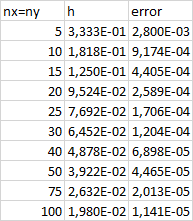
\includegraphics[width=0.8\textwidth]{Lab5/charts/zad2/error_dane.png}
	\end{center}
\end{figure}

\begin{figure}[!ht]
	\begin{center}
		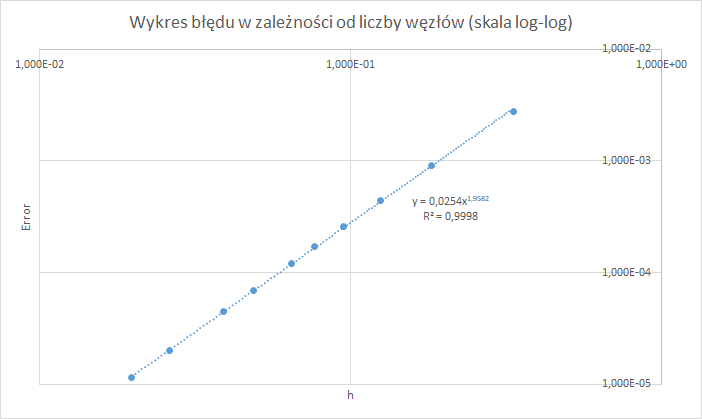
\includegraphics[width=0.8\textwidth]{Lab5/charts/zad2/error.png}
	\end{center}
\end{figure}

\newpage

c)

Dla nx = ny = 5:

\begin{figure}[!ht]
	\begin{center}
		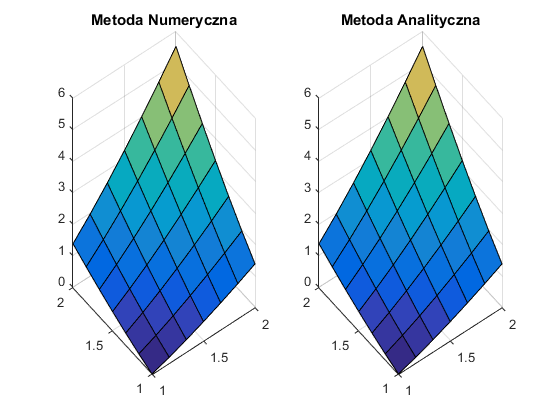
\includegraphics[width=0.78\textwidth]{Lab5/charts/zad3/5x5.png}
	\end{center}
\end{figure}

Czas wykonywania algorytmu $ = 0.0148 s$

Dla nx = ny = 15:

\begin{figure}[!ht]
	\begin{center}
		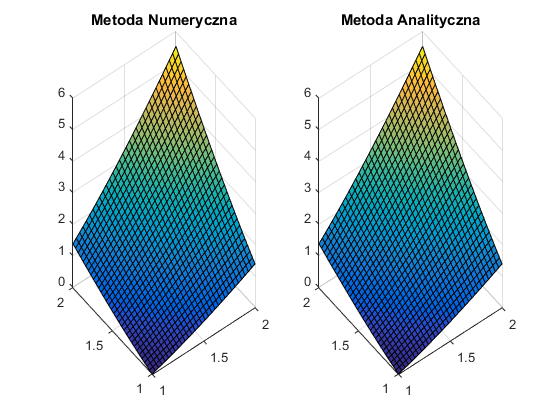
\includegraphics[width=0.78\textwidth]{Lab5/charts/zad3/15x15.png}
	\end{center}
\end{figure}

Czas wykonywania algorytmu $ = 0.0159 s$

\newpage
Dla nx = ny = 30:

\begin{figure}[!ht]
	\begin{center}
		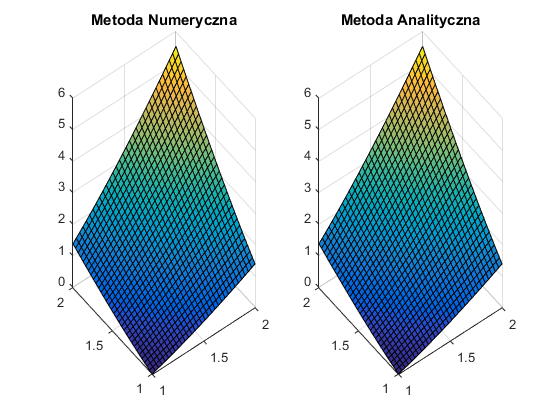
\includegraphics[width=0.8\textwidth]{Lab5/charts/zad3/30x30.png}
	\end{center}
\end{figure}

Czas wykonywania algorytmu $ = 0.0363 s$

Dla nx = ny = 100:

\begin{figure}[!ht]
	\begin{center}
		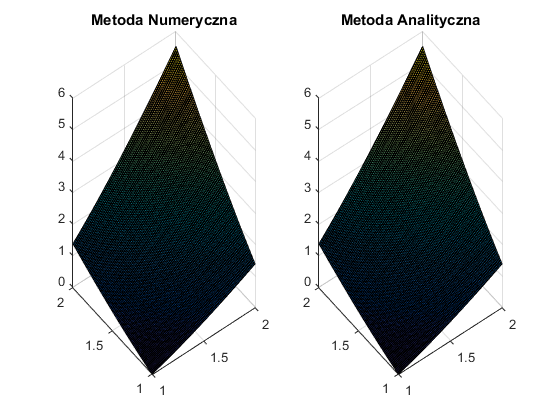
\includegraphics[width=0.8\textwidth]{Lab5/charts/zad3/100x100.png}
	\end{center}
\end{figure}

Czas wykonywania algorytmu $ = 6,538 s$

\newpage

Błąd metody w zależności od liczby węzłów:

\begin{figure}[!ht]
	\begin{center}
		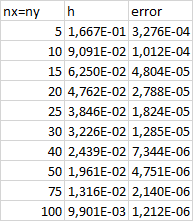
\includegraphics[width=0.8\textwidth]{Lab5/charts/zad3/error_dane.png}
	\end{center}
\end{figure}

\begin{figure}[!ht]
	\begin{center}
		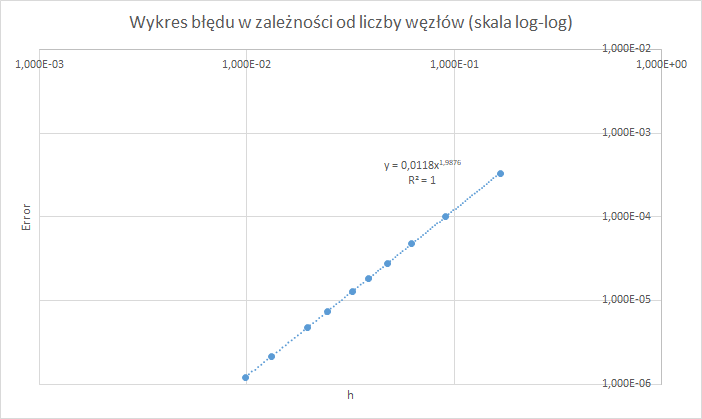
\includegraphics[width=0.8\textwidth]{Lab5/charts/zad3/error.png}
	\end{center}
\end{figure}


\newpage